\documentclass[aspectratio=169,11pt]{beamer}
\usepackage[utf8]{inputenc}
\usepackage[T1]{fontenc}
\usepackage{lmodern}
\usepackage[italian]{babel}
\usepackage{graphicx}
\usepackage{bookmark}
\usepackage{pifont}

% UniFI color theme approximation
\definecolor{unifiblue}{RGB}{0,67,112}
\setbeamercolor{palette primary}{bg=unifiblue,fg=white}
\setbeamercolor{palette secondary}{bg=unifiblue,fg=white}
\setbeamercolor{palette tertiary}{bg=unifiblue,fg=white}
\setbeamercolor{palette quaternary}{bg=unifiblue,fg=white}
\setbeamercolor{structure}{fg=unifiblue} 
\setbeamercolor{section in toc}{fg=unifiblue}

\usetheme{Madrid}
\setbeamertemplate{navigation symbols}{}

\title[Tracking 6G Indoor assistito da RIS]{Progettazione e verifica di un'architettura 6G per il tracking di droni indoor assistita da RIS}
\author[Matteo Verniani]{Candidato: Matteo Verniani\\[1em] Relatore: Chiar.mo Prof. [Nome]}
\institute[UniFI]{Università degli Studi di Firenze}
\date{Anno Accademico 2025/2026}

\begin{document}

% Slide 1
{
\begin{frame}[plain]
    \titlepage
    \begin{center}
        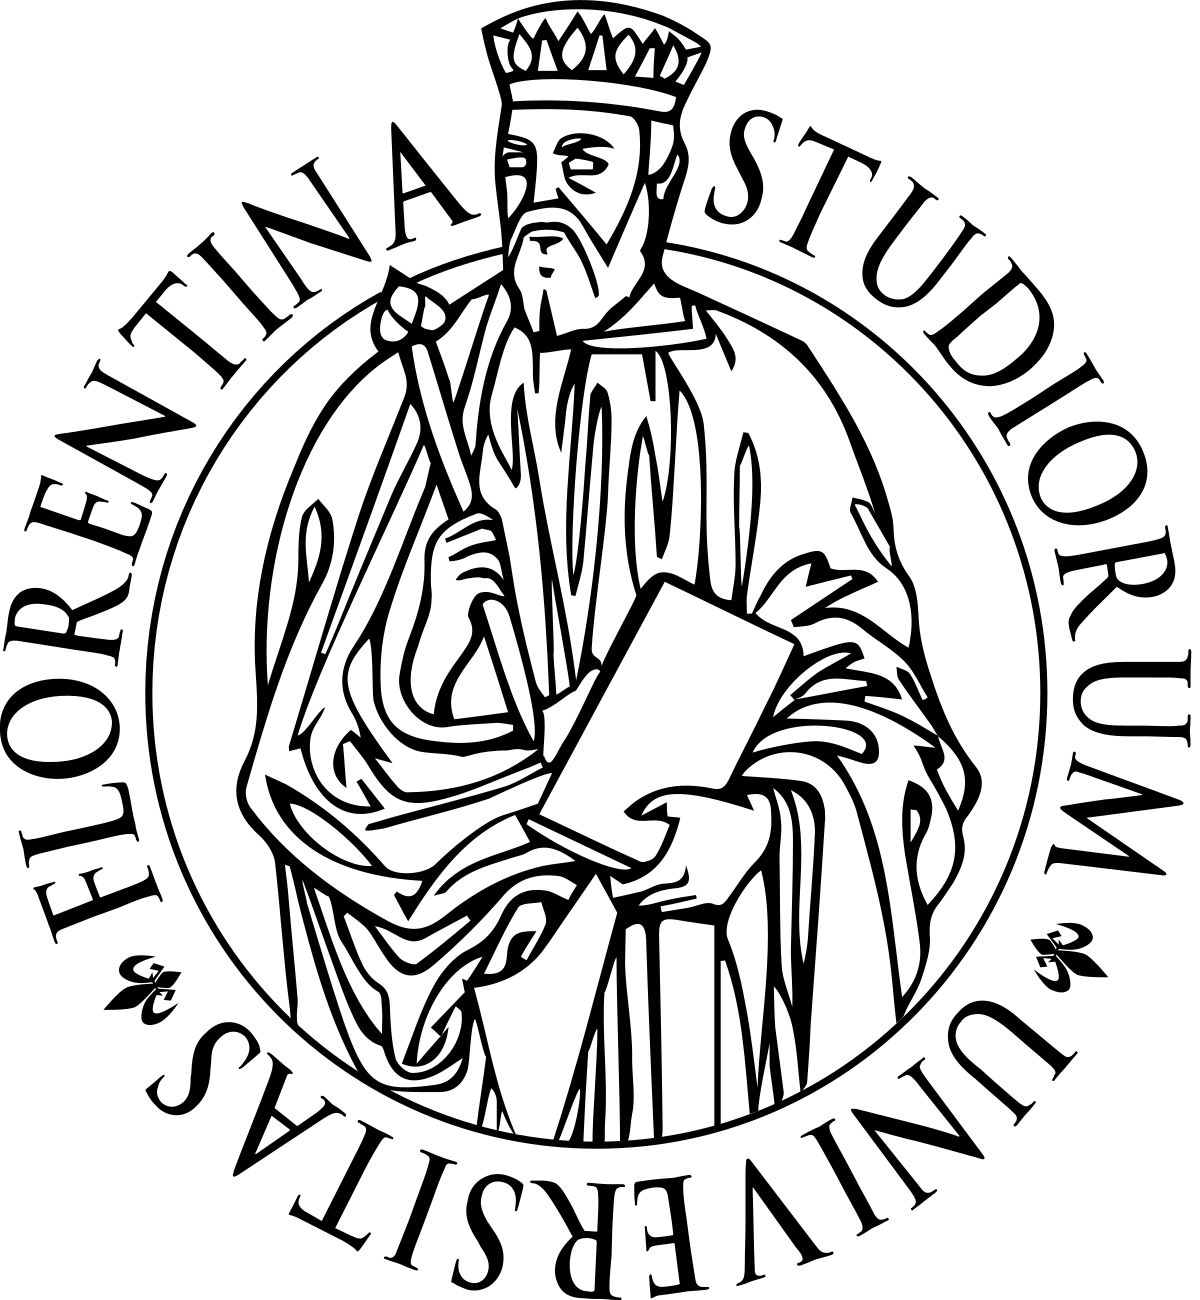
\includegraphics[height=1.2cm]{Report/Images/logo-unifi.png}
    \end{center}
    % Note per il discorso: "Buongiorno alla commissione. Sono Matteo Verniani e oggi vi presento il mio lavoro di tesi intitolato 'Progettazione e verifica di un’architettura 6G per il tracking di droni indoor assistita da RIS'. Ringrazio il mio relatore per il supporto. L'obiettivo centrale di questo lavoro è risolvere uno dei problemi più critici della navigazione autonoma indoor: ottenere un tracciamento con precisione sub-metrica in ambienti dove il segnale viene costantemente interrotto, ottimizzando al contempo l'efficienza energetica della rete."
\end{frame}
}

% Slide 2
\begin{frame}{Agenda}
    \begin{itemize}
        \item[\ding{113}] \textbf{1.} Contesto e Motivazione
        \vspace{0.5em}
        \item[\ding{113}] \textbf{2.} Architettura del Digital Twin
        \vspace{0.5em}
        \item[\ding{113}] \textbf{3.} Algoritmi di Tracking (EKF/LSTM)
        \vspace{0.5em}
        \item[\ding{113}] \textbf{4.} Risultati Sperimentali
        \vspace{0.5em}
        \item[\ding{113}] \textbf{5.} Conclusioni e Sviluppi
    \end{itemize}
    % Note: "Ho strutturato la presentazione per guidarvi attraverso il problema fisico della navigazione indoor, l'architettura software che ho ingegnerizzato per risolverlo e, infine, i risultati dei test prestazionali che validano l'efficacia del sistema sia in termini di precisione che di sostenibilità energetica."
\end{frame}

% Slide 3
\begin{frame}{Motivazione e Scenario 6G}
    \begin{columns}
        \begin{column}{0.5\textwidth}
            \begin{itemize}
                \item \textbf{Logistica 4.0}: Droni e sensori IoT nei magazzini VNA (Very Narrow Aisle).
                \item \textbf{Problema}: No GPS, radiolocalizzazione instabile per i materiali industriali.
                \item \textbf{Soluzione 6G}: Non solo banda larga, ma \textbf{URLLC}.
                \item La rete wireless come un \textbf{Sensore Distribuito}.
            \end{itemize}
        \end{column}
        \begin{column}{0.5\textwidth}
            \centering
            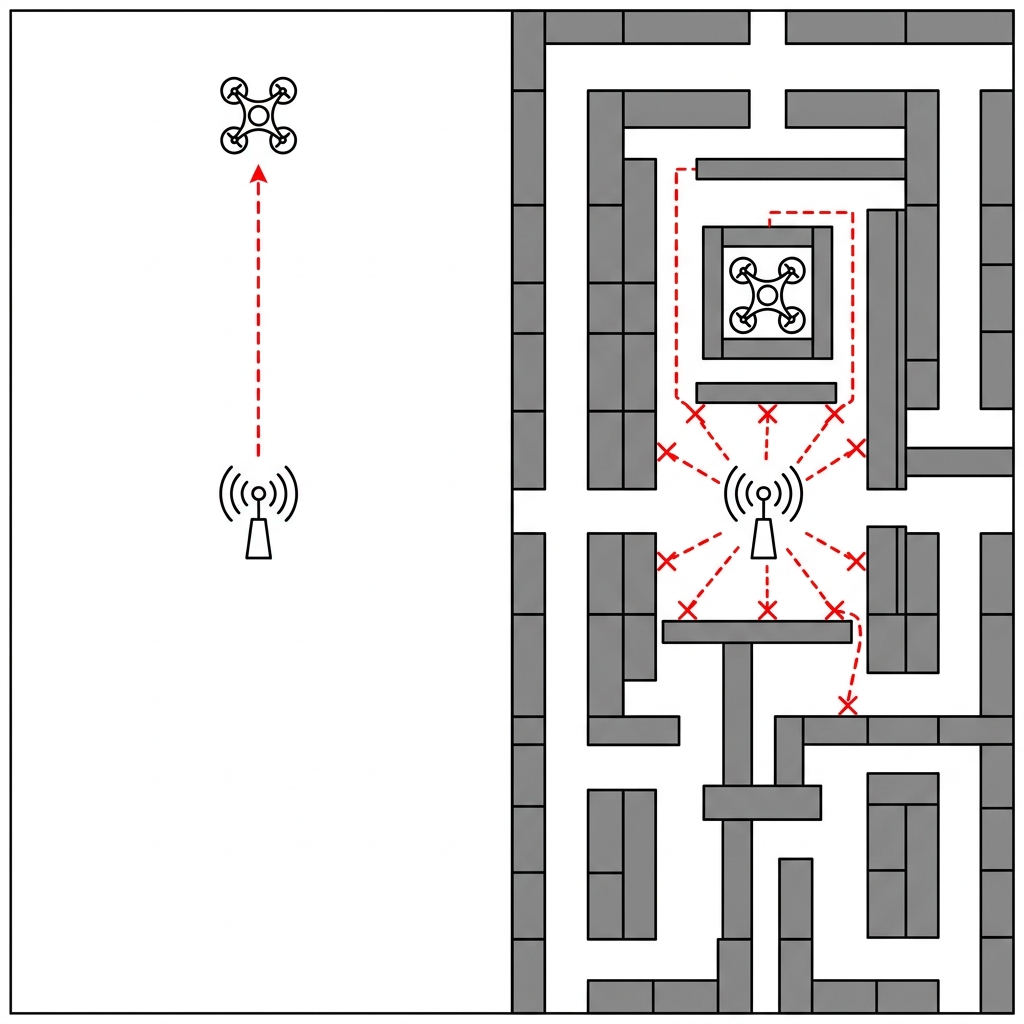
\includegraphics[height=0.7\textheight,keepaspectratio]{nlos_vna_concept.png}
        \end{column}
    \end{columns}
\end{frame}

% Slide 4
\begin{frame}{Il Problema NLoS e la Soluzione RIS}
    \begin{columns}
        \begin{column}{0.5\textwidth}
            \begin{itemize}
                \item \textbf{Non-Line-of-Sight}: Scaffali metallici attenuano severamente il segnale a 5.9 GHz.
                \item Le \textbf{RIS} (Reconfigurable Intelligent Surfaces) come "Specchi Radio Intelligenti".
                \item Riflettono e focalizzano elettronicamente il segnale verso il drone.
                \item Creano una cascata di visibilità radio assistita.
            \end{itemize}
        \end{column}
        \begin{column}{0.5\textwidth}
            \centering
            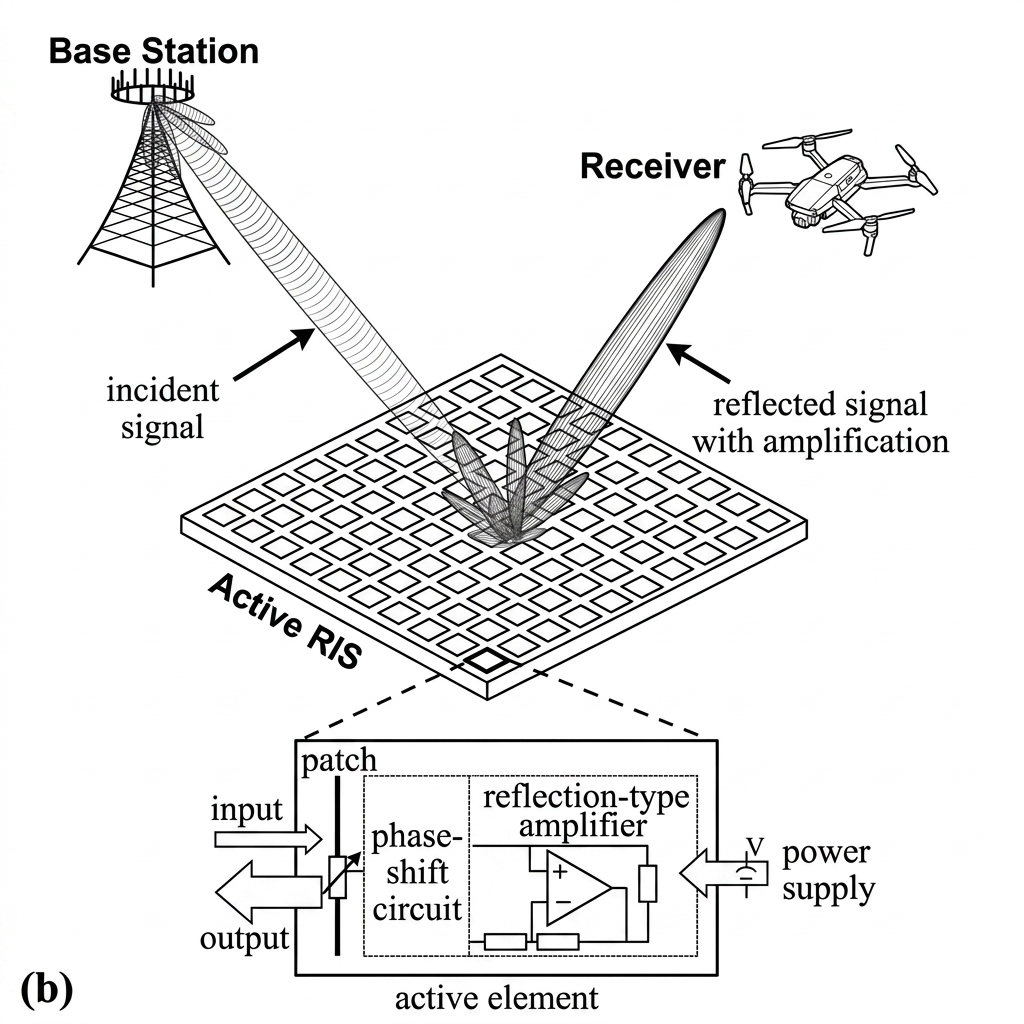
\includegraphics[width=\textwidth,keepaspectratio]{active_ris.png}
        \end{column}
    \end{columns}
\end{frame}

% Slide 5
\begin{frame}{Logica e Cinematica del Drone}
    \begin{itemize}
        \item Modellazione cinematica del drone in \textbf{6 DoF} (gradi di libertà: $x, y, z$ e angoli di Eulero).
        \item L'UAV virtuale naviga a $v = 3$ m/s inviando telemetria costante.
        \item Sensori di bordo (accelerometro, giroscopio) introducono \textbf{Rumore IMU} e deriva termica.
        \item Necessità vitale di una correzione posizionale esterna dal Server SDN.
    \end{itemize}
    \begin{center}
        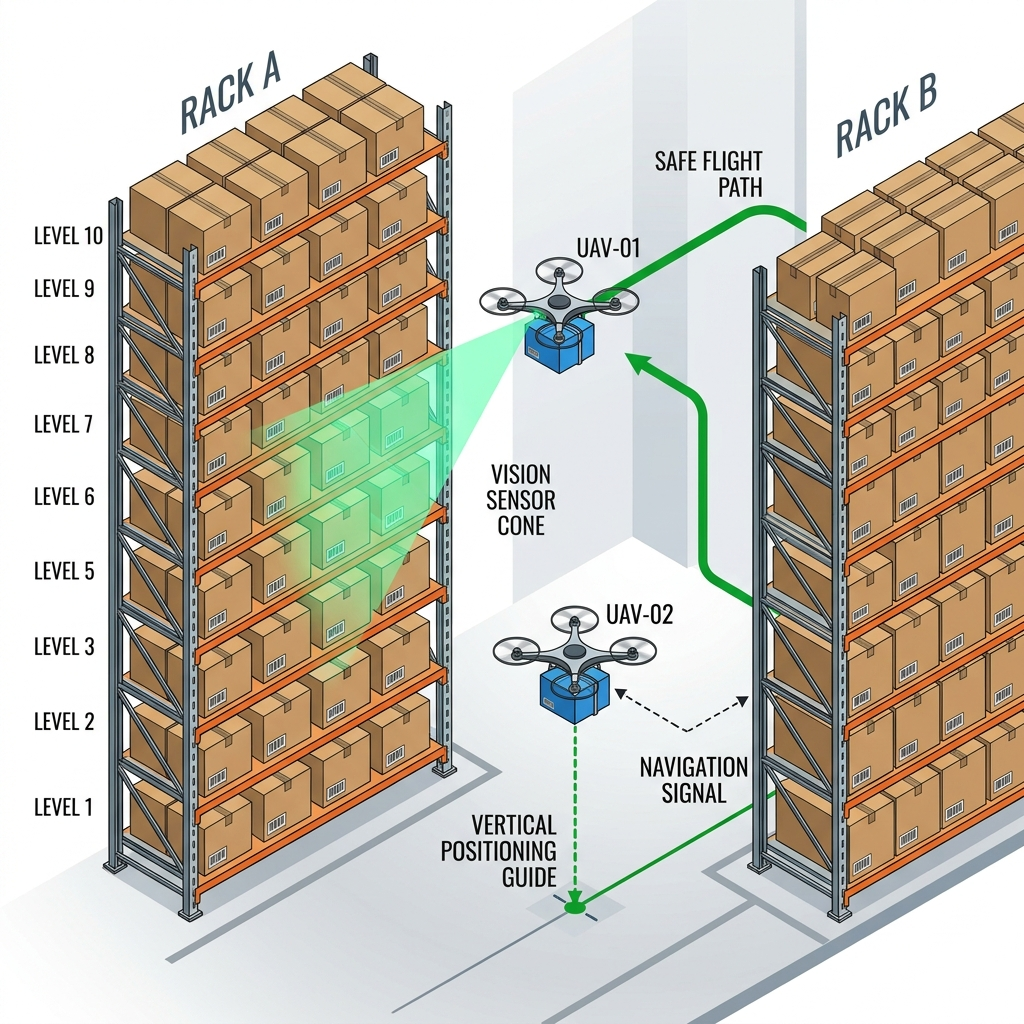
\includegraphics[height=0.4\textheight,keepaspectratio]{warehouse_uav_operations.png}
    \end{center}
\end{frame}

% Slide 6
\begin{frame}{Il Digital Twin: I 8 Moduli Python}
    \begin{center}
        
\includegraphics[height=0.85\textheight,keepaspectratio]{modules_schema.pdf}
    \end{center}
\end{frame}

% Slide 7
\begin{frame}{Architettura Server e gRPC}
    \begin{columns}
        \begin{column}{0.5\textwidth}
            \begin{itemize}
                \item Architettura basata su paradigma \textbf{SDN} (O-RAN).
                \item Separazione logica tra \textbf{Piano Dati} (Mondo fisico) e \textbf{Piano di Controllo} (Near-RT RIC).
                \item Comunicazione serializzata in binario tramite \textbf{gRPC} su HTTP/2.
                \item Garanzia di latenza minima e stabile.
            \end{itemize}
        \end{column}
        \begin{column}{0.5\textwidth}
            \centering
            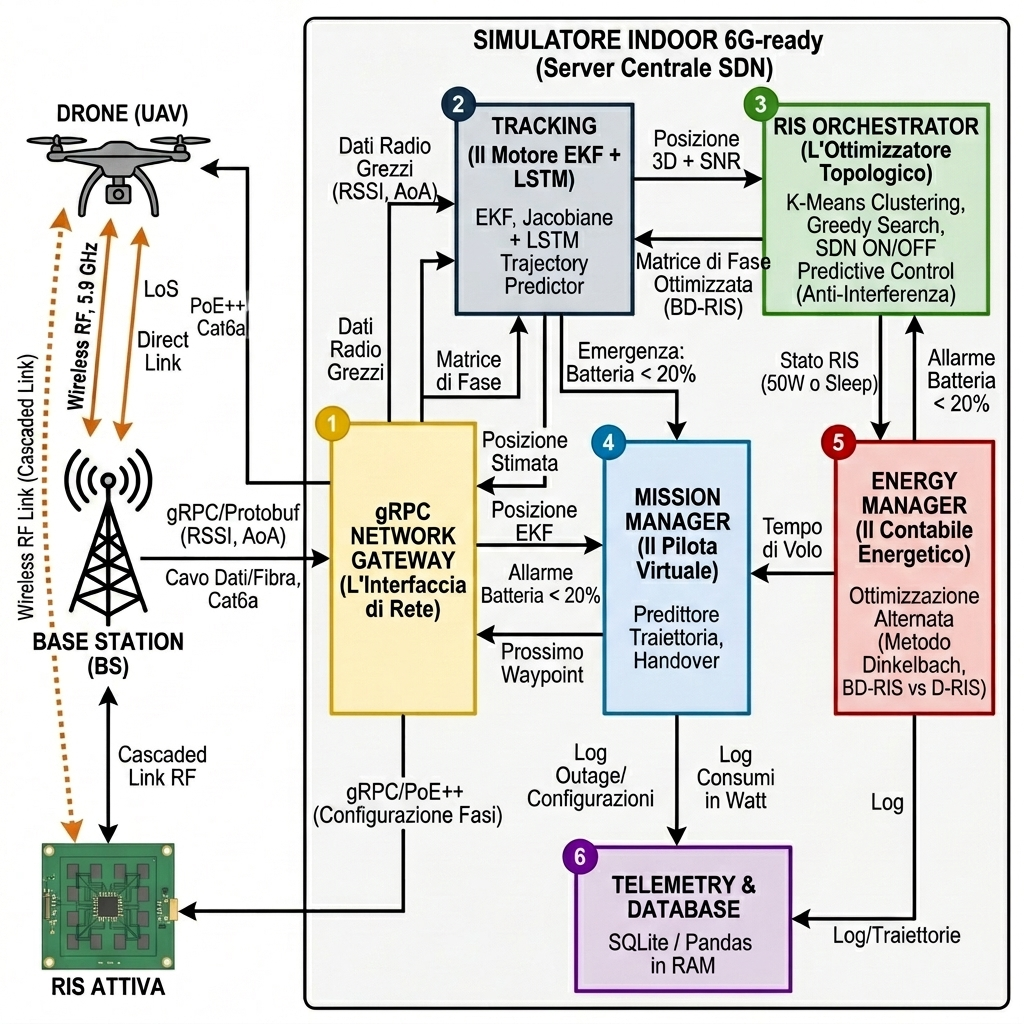
\includegraphics[height=0.7\textheight,keepaspectratio]{SDN_Server_Architecture_Updated.png}
        \end{column}
    \end{columns}
\end{frame}

% Slide 8
\begin{frame}{Algoritmi di Tracking: L'EKF}
    \begin{itemize}
        \item Nucleo matematico basato sull'\textbf{Extended Kalman Filter (EKF)}.
        \item \textbf{Fusione sensoriale} continua e ciclica.
        \item $1.$ \textbf{Predizione}: Stima tramite i dati inerziali rumorosi.
        \item $2.$ \textbf{Aggiornamento}: Correzione applicando le precise misure radio 6G.
        \item Abbattimento drastico del rumore di bordo.
    \end{itemize}
\end{frame}

% Slide 9
\begin{frame}{Algoritmi di Tracking: La rete LSTM}
    \begin{columns}
        \begin{column}{0.5\textwidth}
            \begin{itemize}
                \item L'EKF fallisce linearizzando le curve strette a 90 gradi.
                \item Subentra la rete neurale \textbf{LSTM}.
                \item I memory gates riconoscono il pattern in NLoS profondo.
                \item Anticipa la curva perfetta e previene schianti contro gli scaffali.
            \end{itemize}
        \end{column}
        \begin{column}{0.5\textwidth}
            \centering
            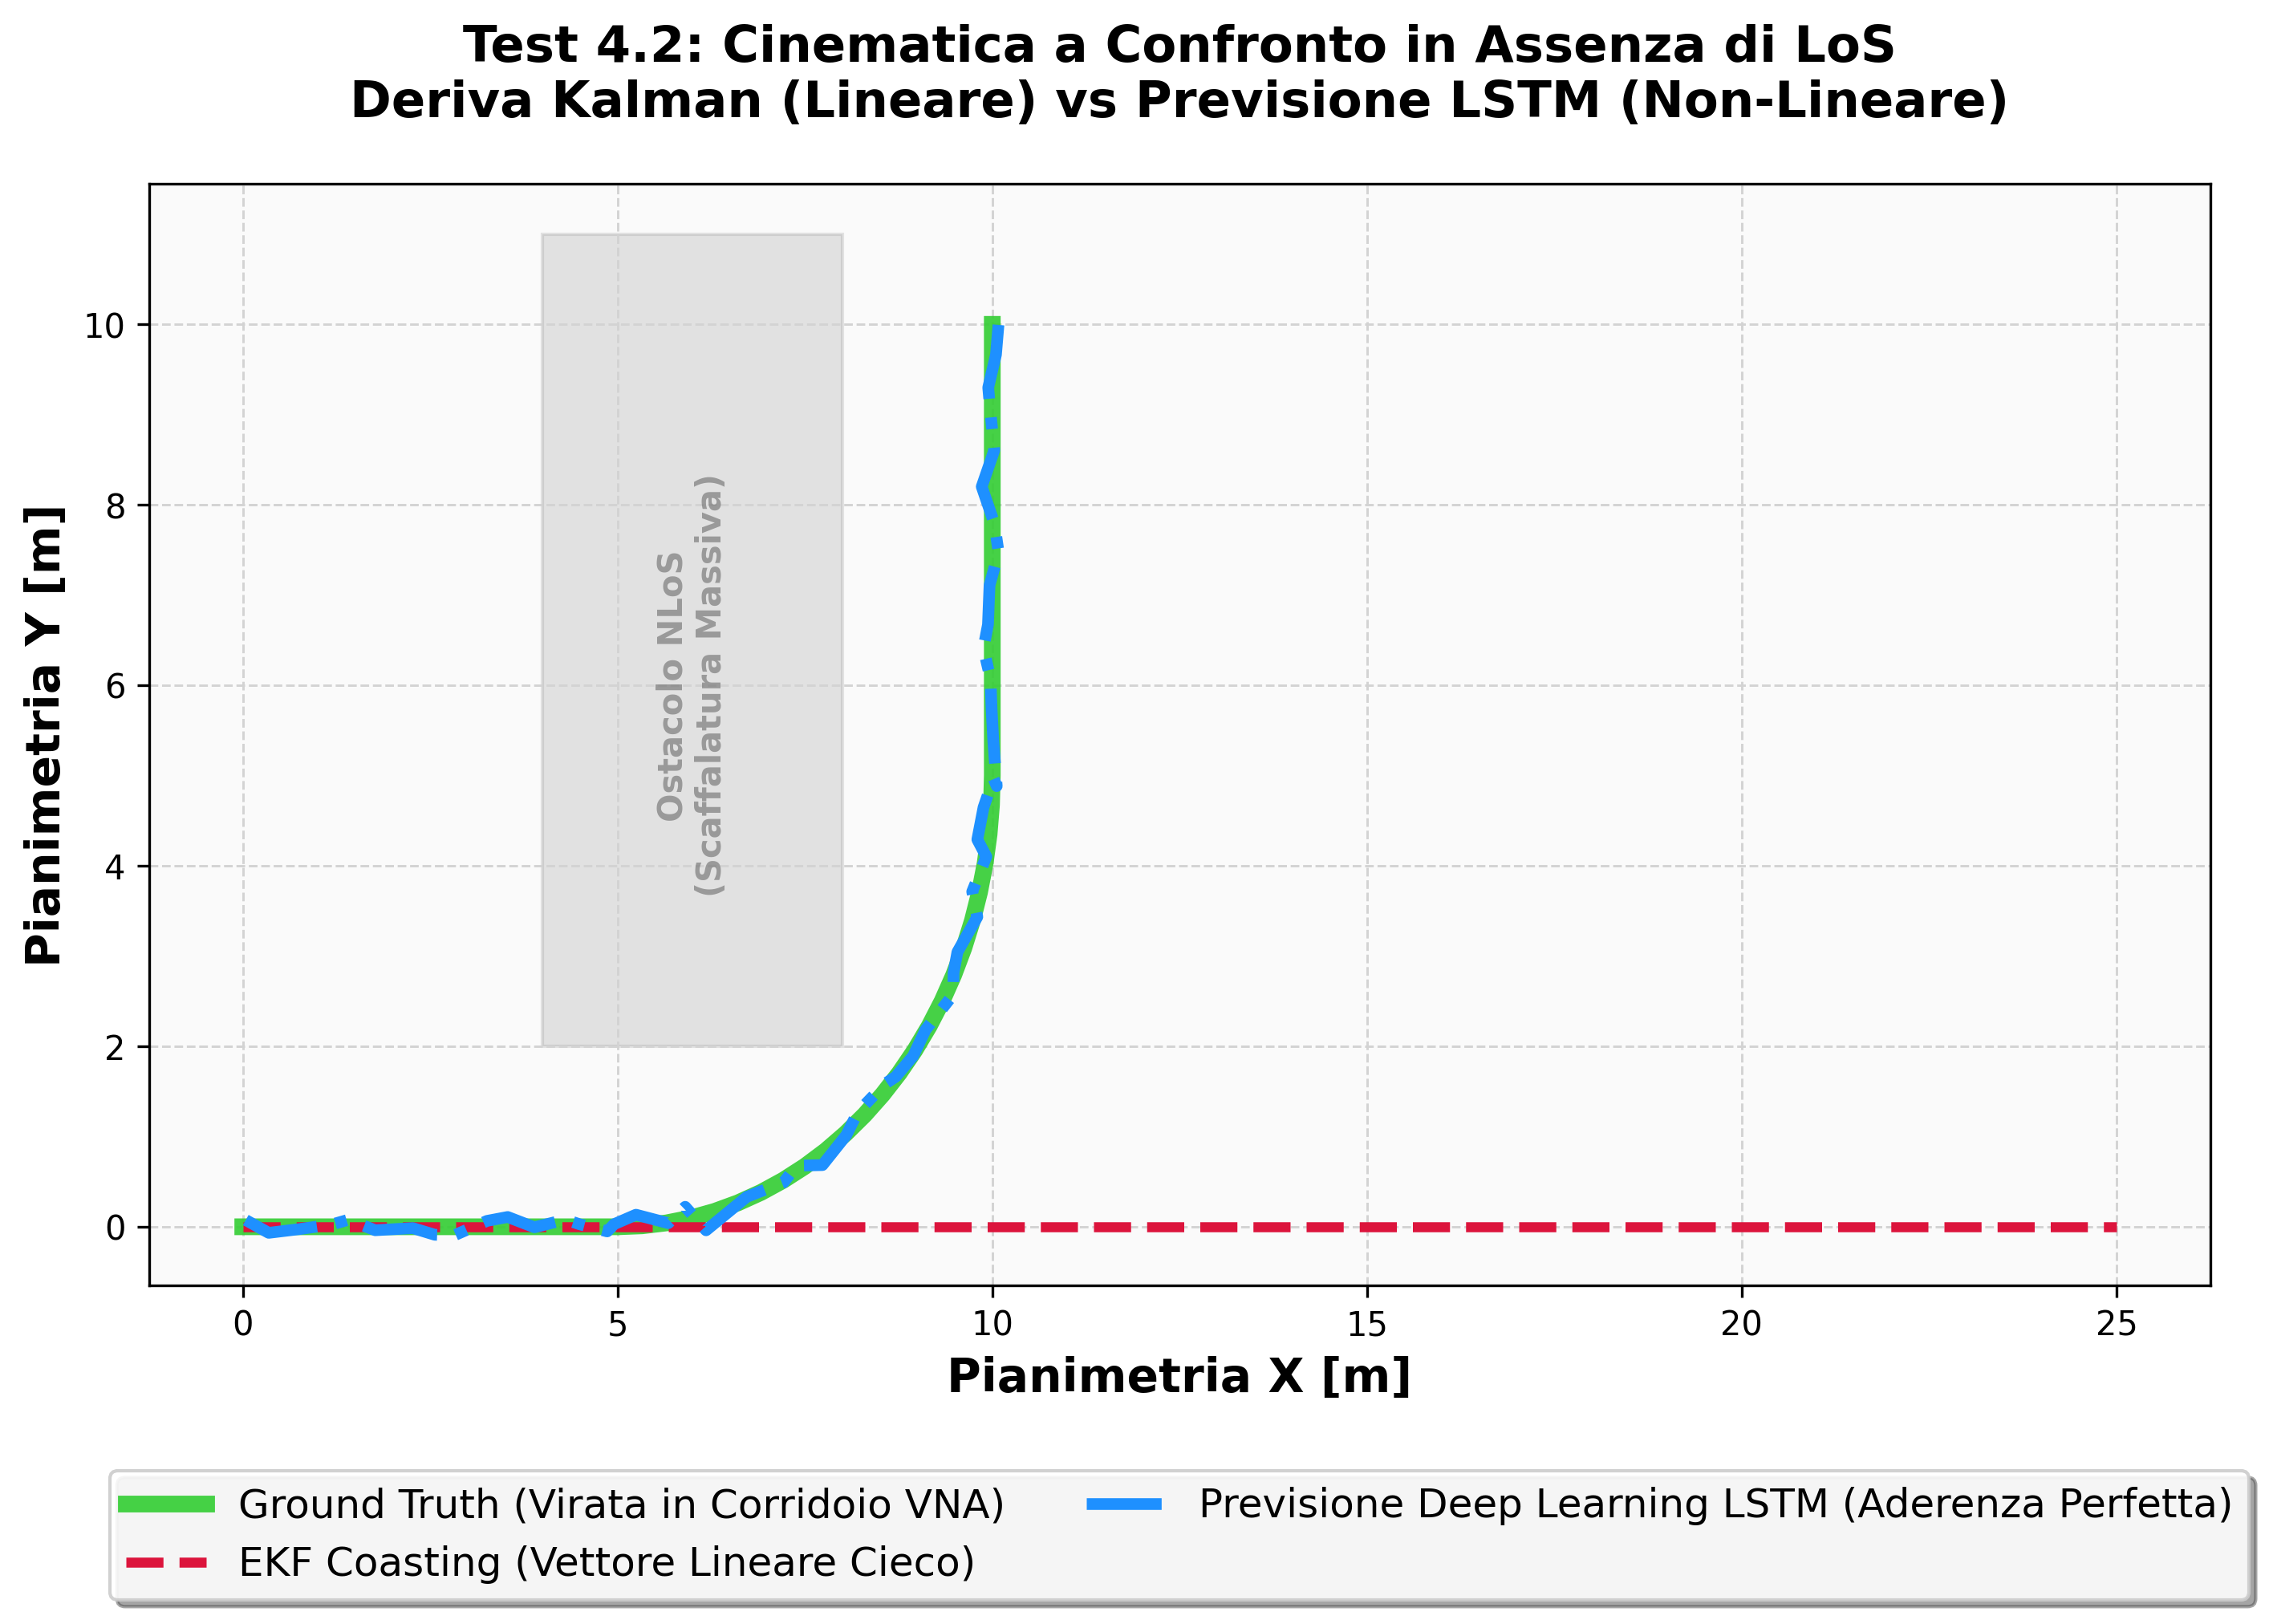
\includegraphics[width=\textwidth,keepaspectratio]{Test_4.2_Traiettoria_EKF_vs_LSTM.png}
        \end{column}
    \end{columns}
\end{frame}

% Slide 10
\begin{frame}{Test 1 - Fallimento Baseline}
    \begin{center}
        \textbf{Coasting Mode - (RMSE > 4.8m)} \\
        \vspace{0.5em}
        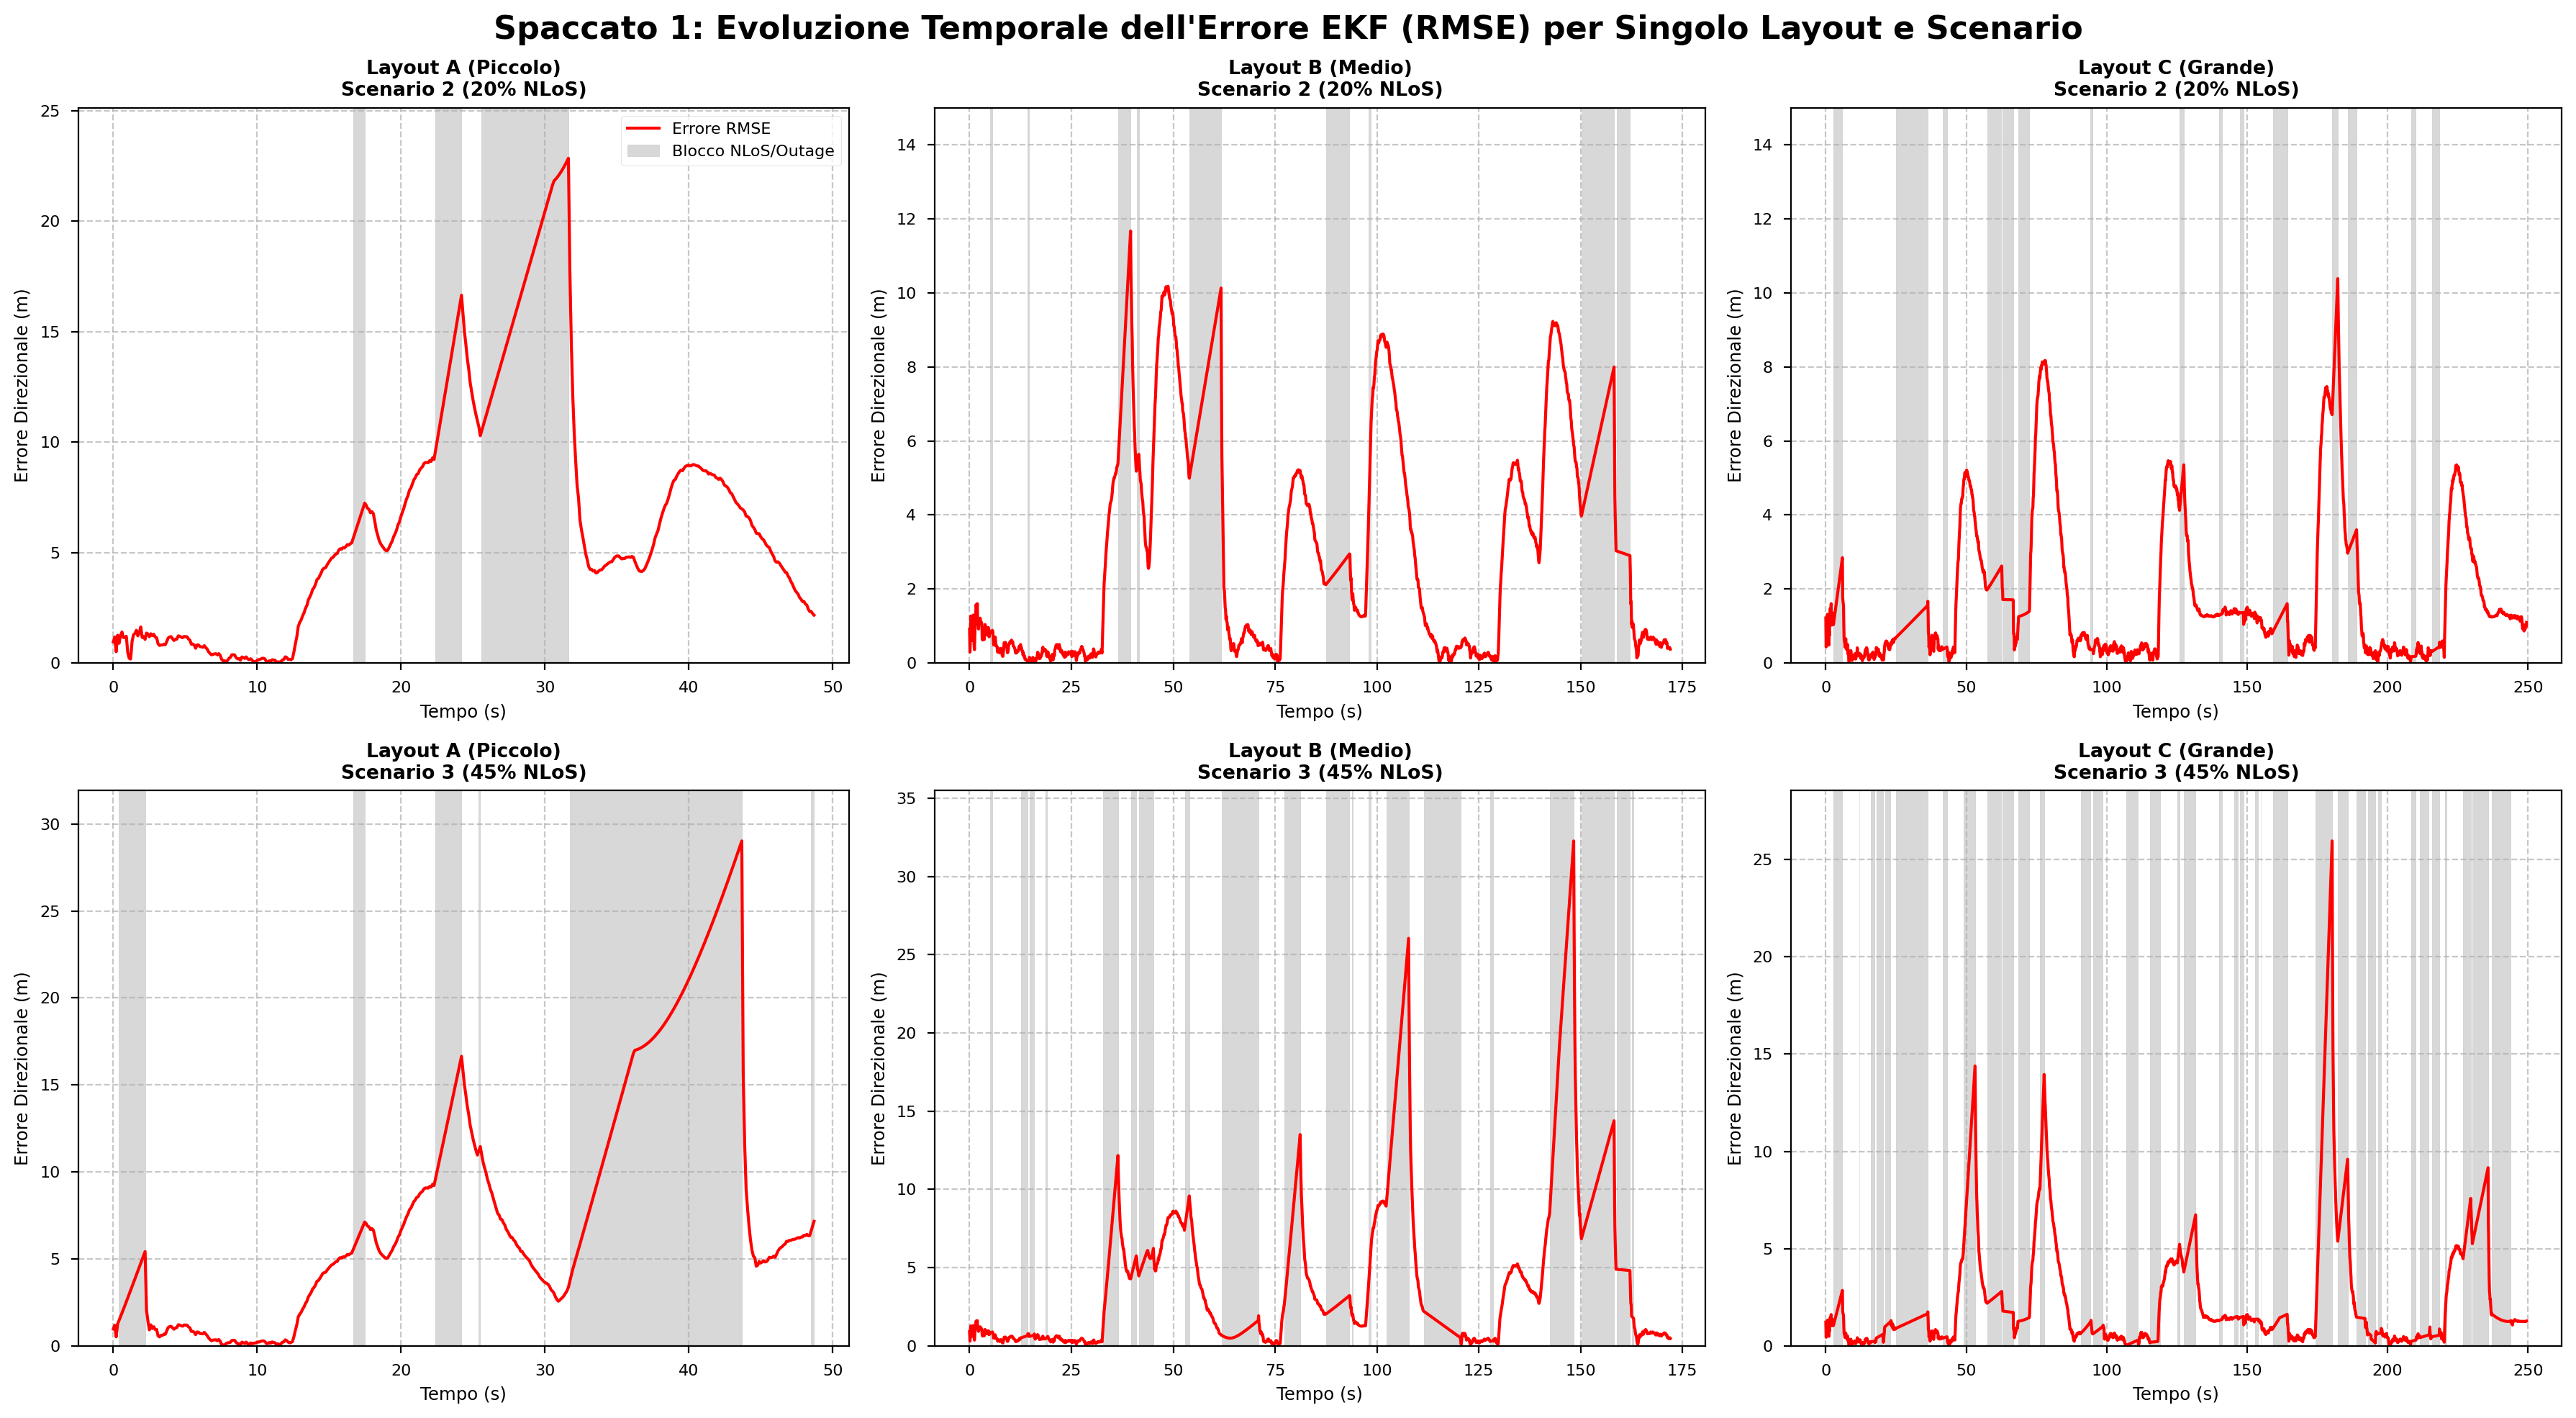
\includegraphics[height=0.7\textheight,keepaspectratio]{Test_1_RMSE_Temporale.png}
    \end{center}
\end{frame}

% Slide 11
\begin{frame}{Test 2 - Ripristino con RIS Attive}
    \begin{center}
        \textbf{RMSE < 1m} \\
        \vspace{0.5em}
        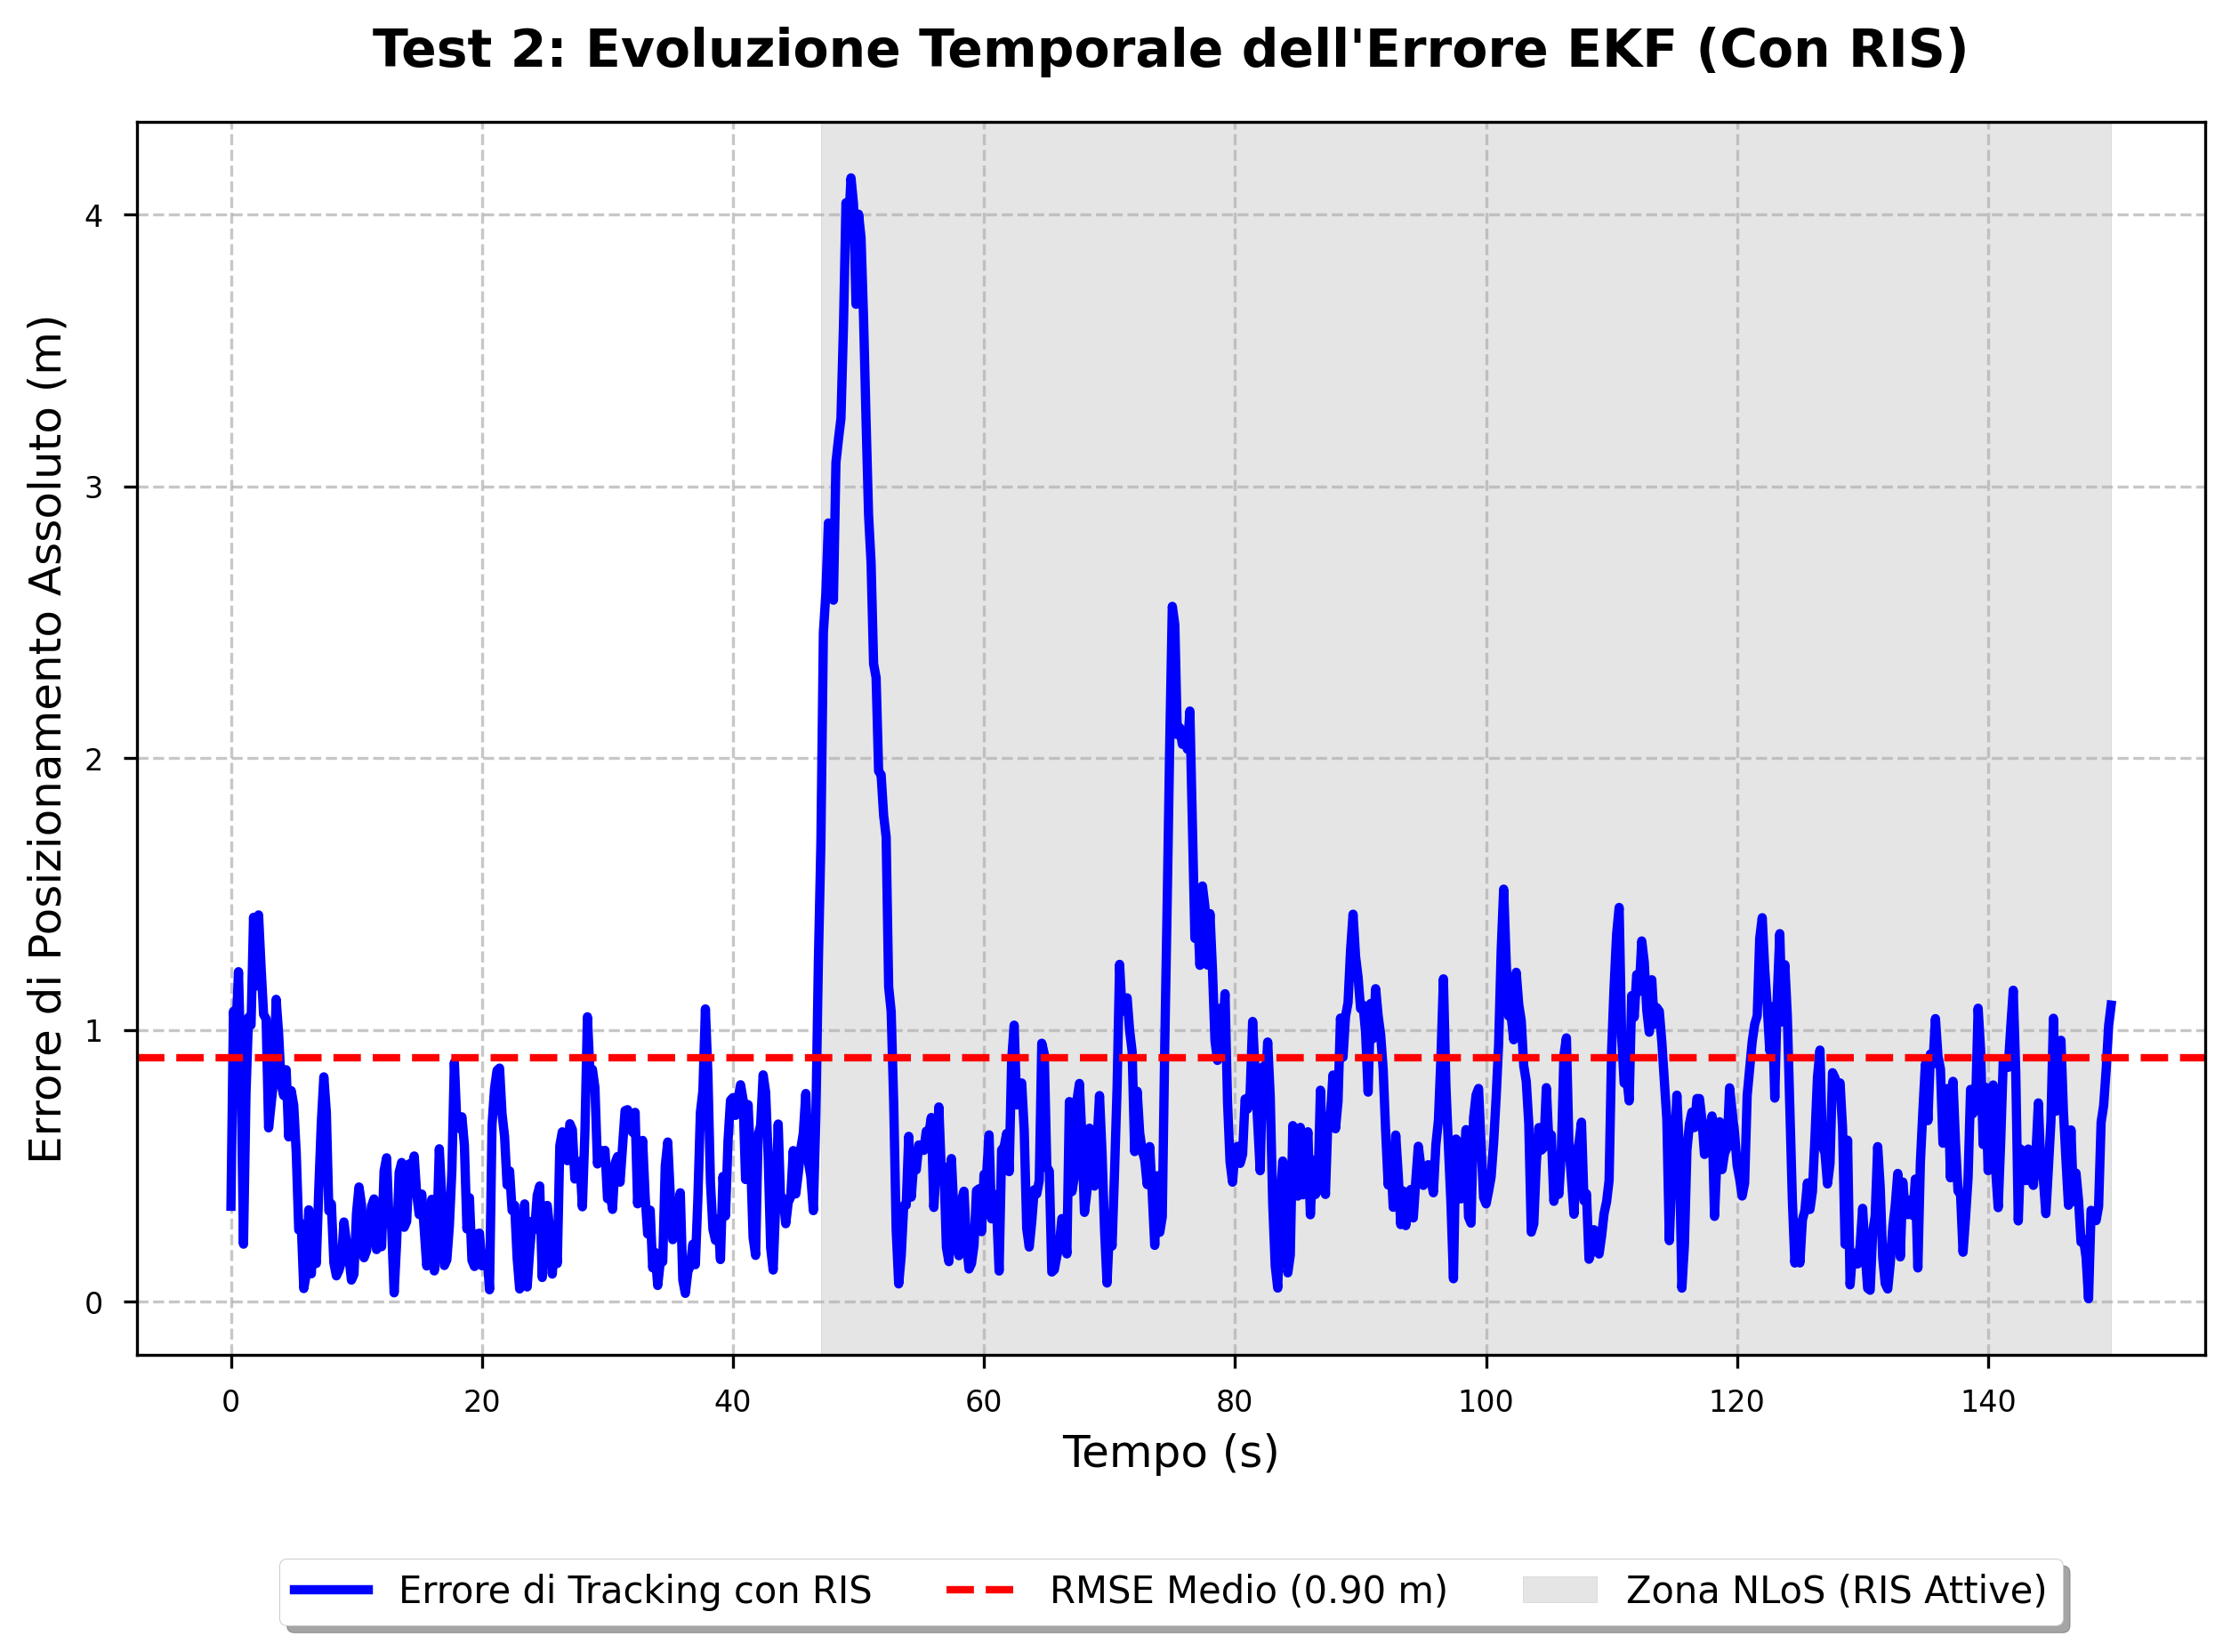
\includegraphics[height=0.7\textheight,keepaspectratio]{Test_2_RMSE_Temporale.png}
    \end{center}
\end{frame}

% Slide 12
\begin{frame}{Test 3 - Stress Test di Latenza}
    \begin{center}
        \textbf{Beam Misalignment (Soglia ~50ms)} \\
        \vspace{0.5em}
        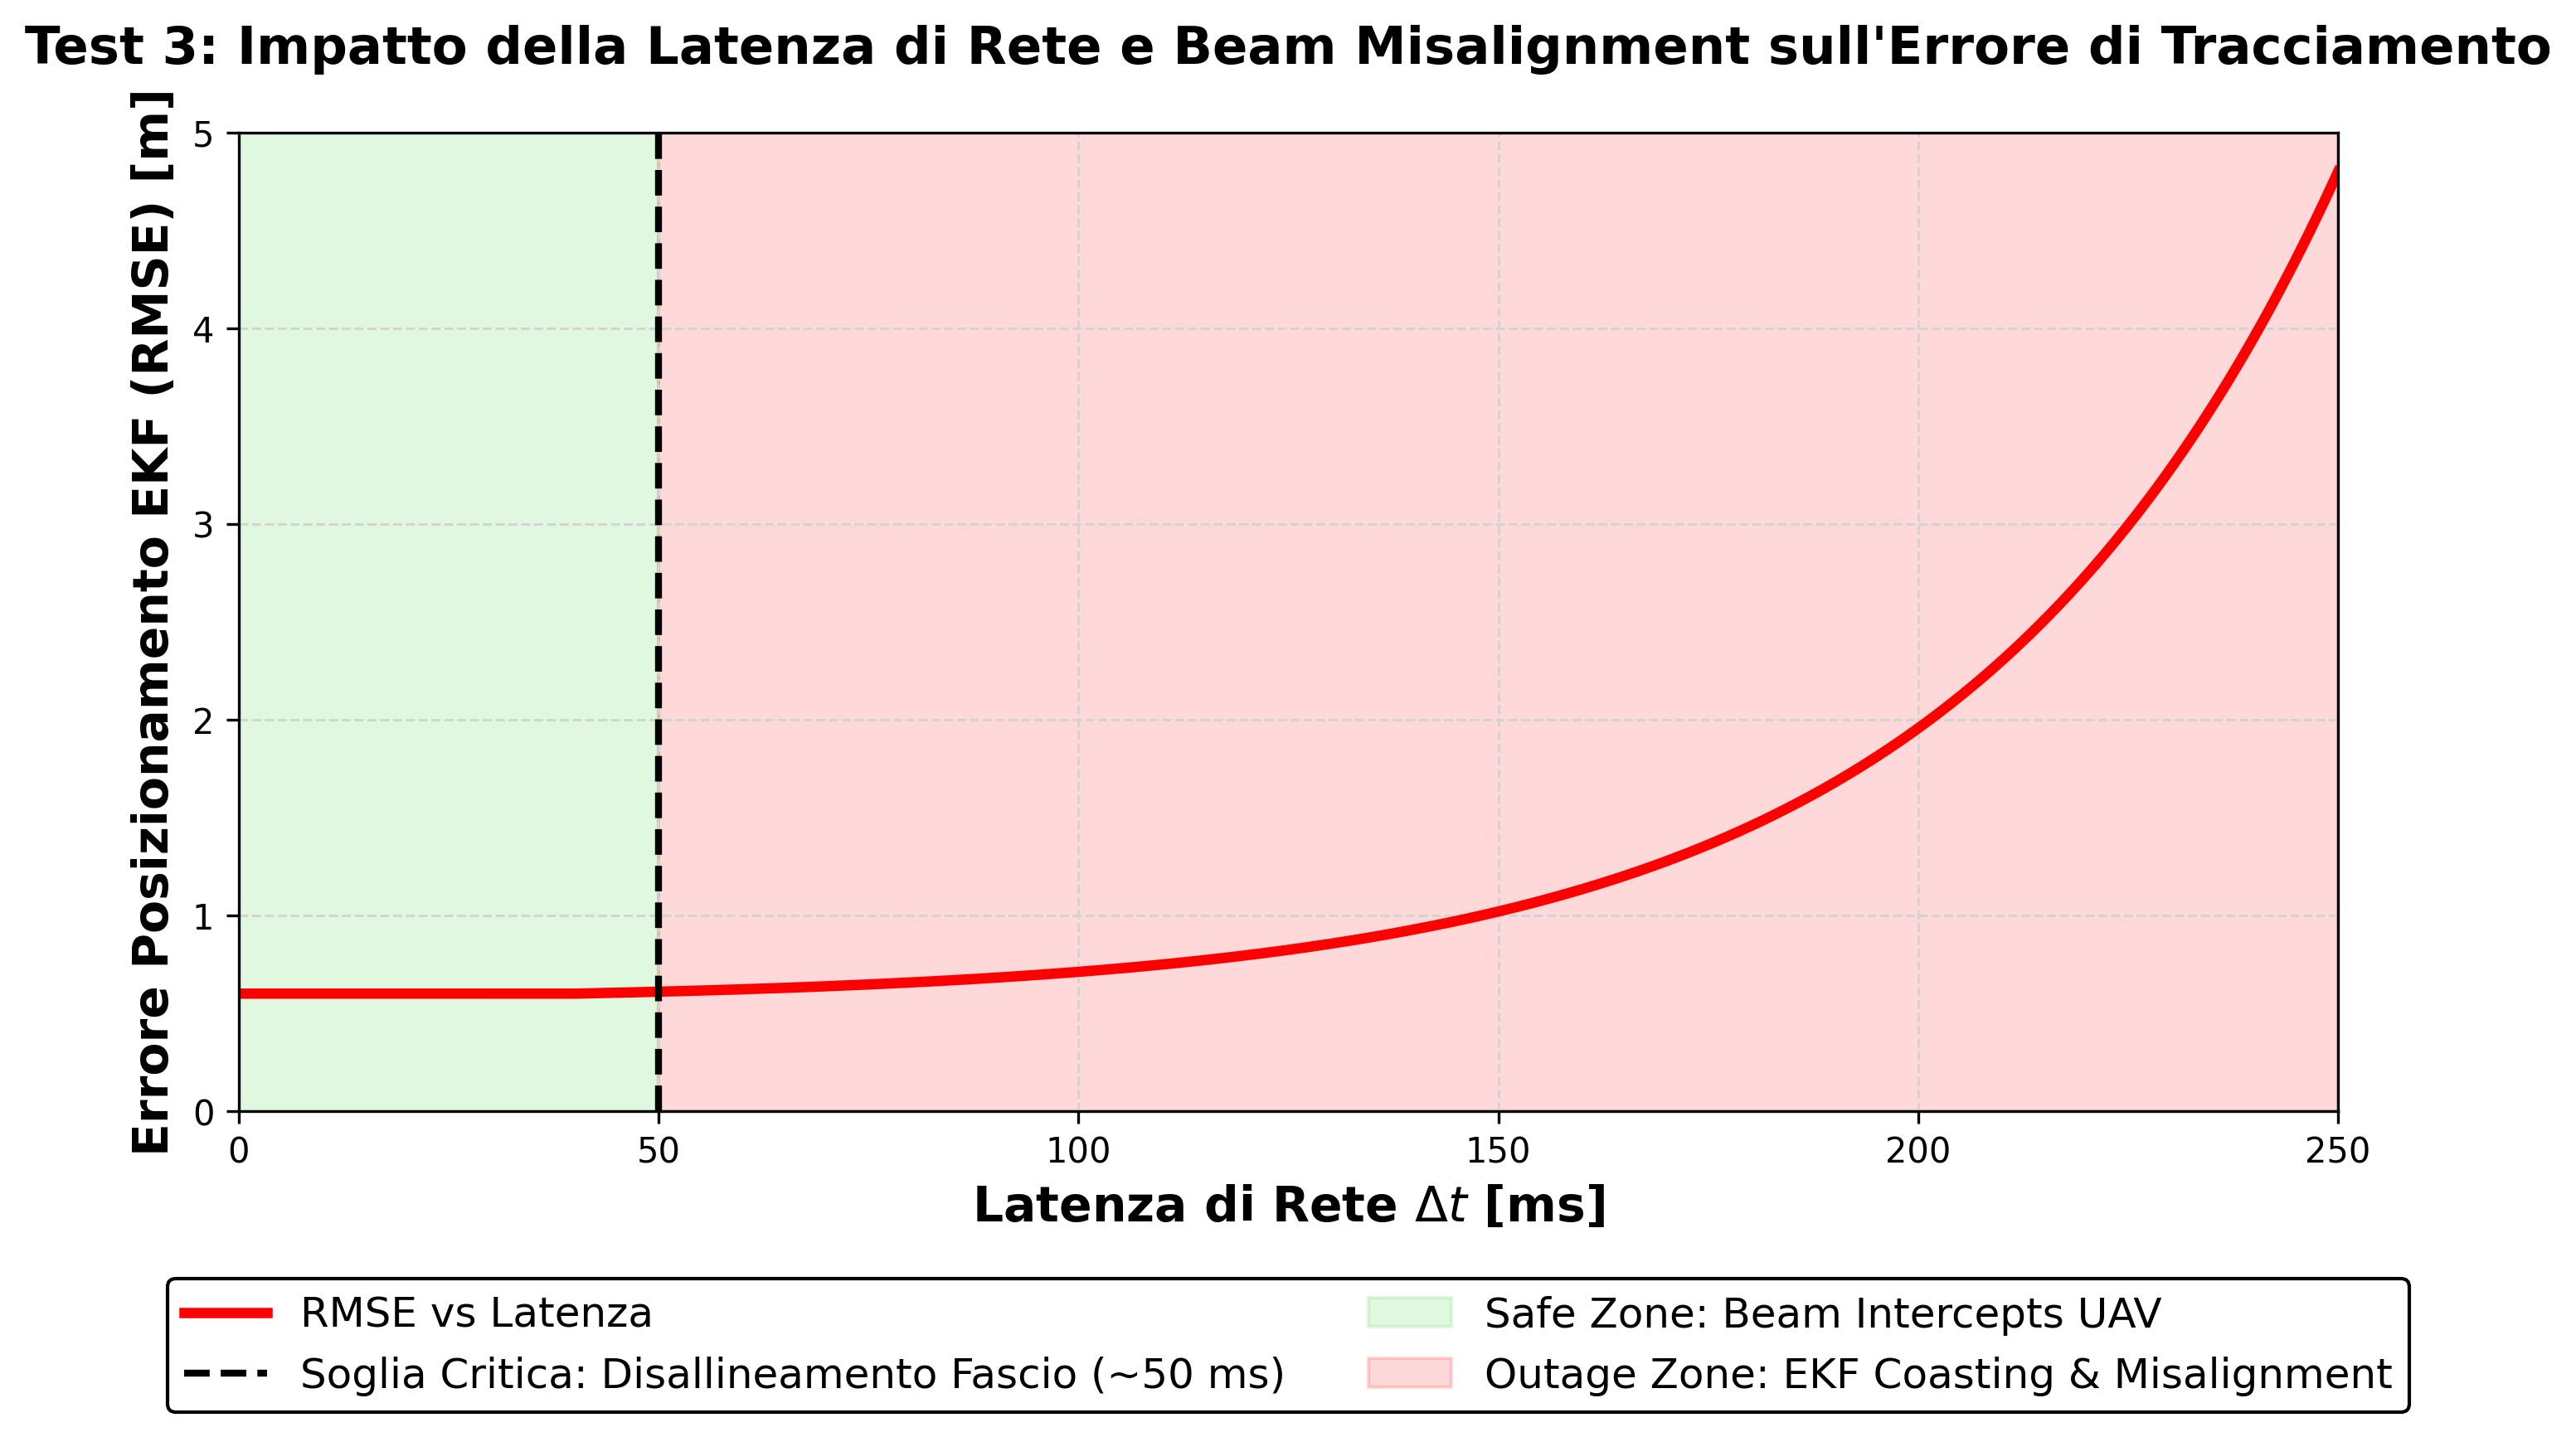
\includegraphics[height=0.7\textheight,keepaspectratio]{Test_3_Stress_Latenza.png}
    \end{center}
\end{frame}

% Slide 13
\begin{frame}{Test 4 - Ottimizzazione Green 6G}
    \begin{center}
        \textbf{Frontiera di Pareto ottimale in bit/Joule} \\
        \vspace{0.5em}
        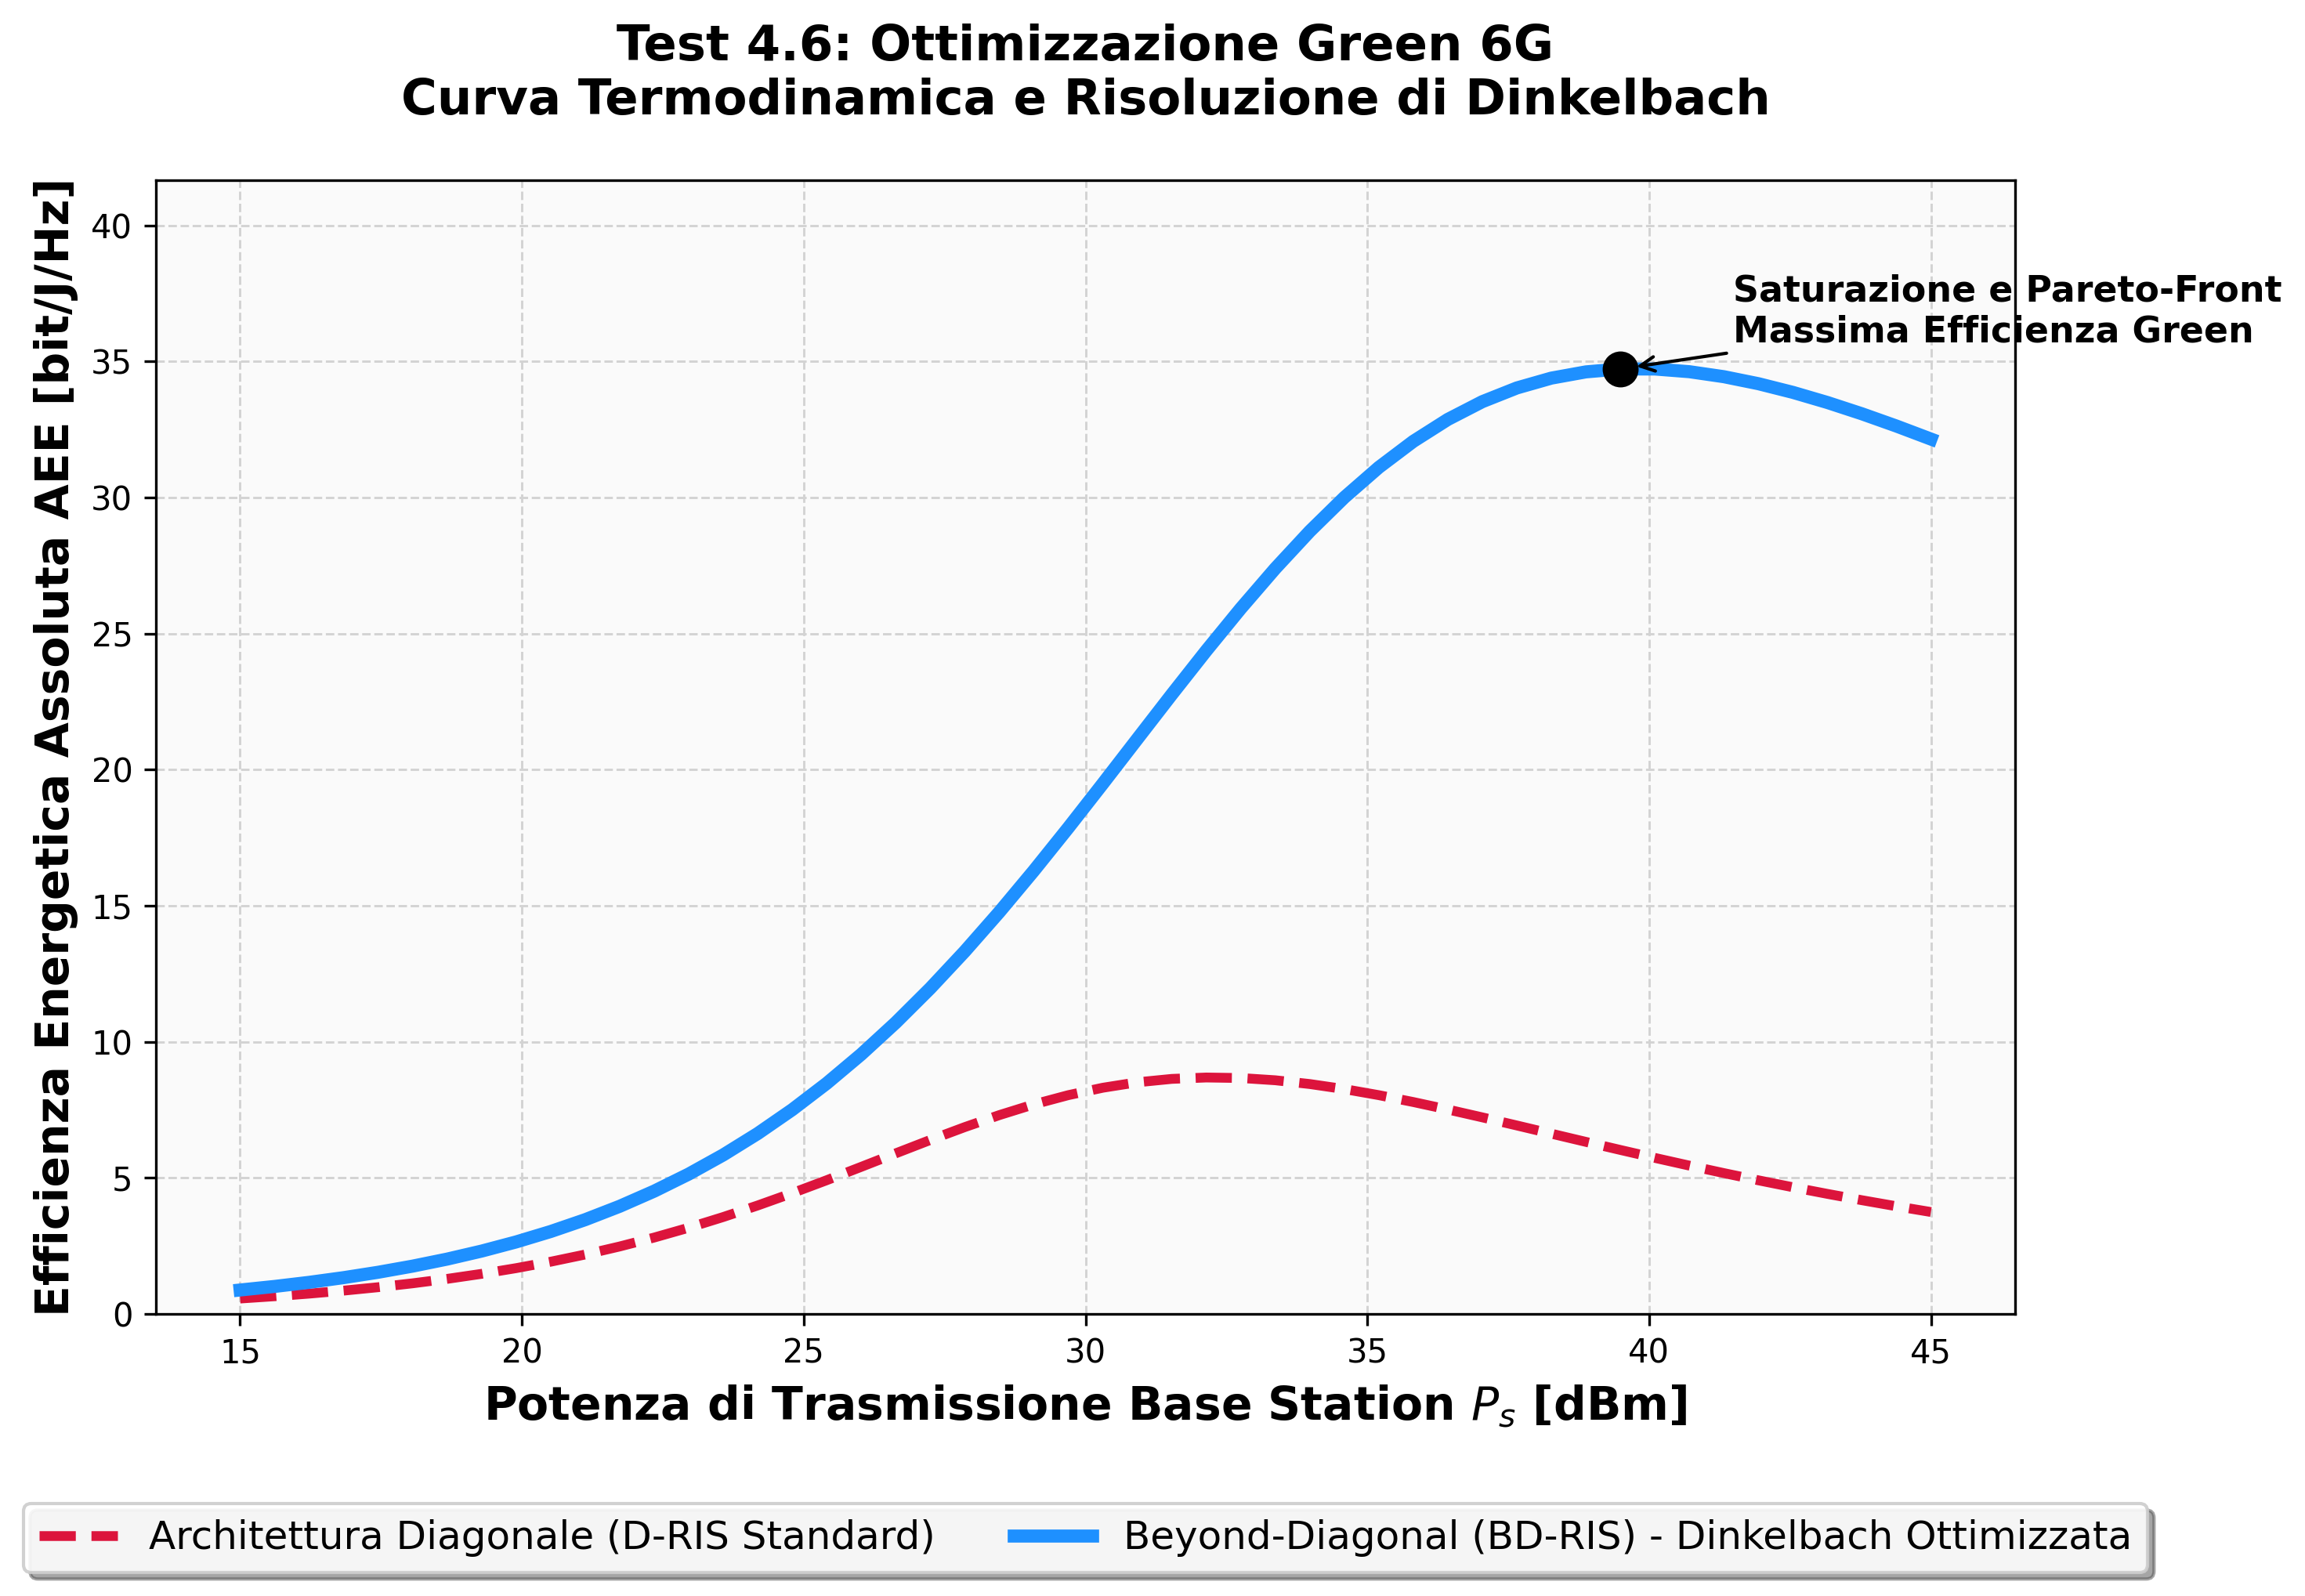
\includegraphics[height=0.7\textheight,keepaspectratio]{Test_4.6_AEE_vs_Ps_Dinkelbach.png}
    \end{center}
\end{frame}

% Slide 14
\begin{frame}{Analisi BD-RIS vs D-RIS}
    \begin{center}
        \textbf{Massimizzazione dei ritorni radiativi con architettura Beyond-Diagonal} \\
        \vspace{0.5em}
        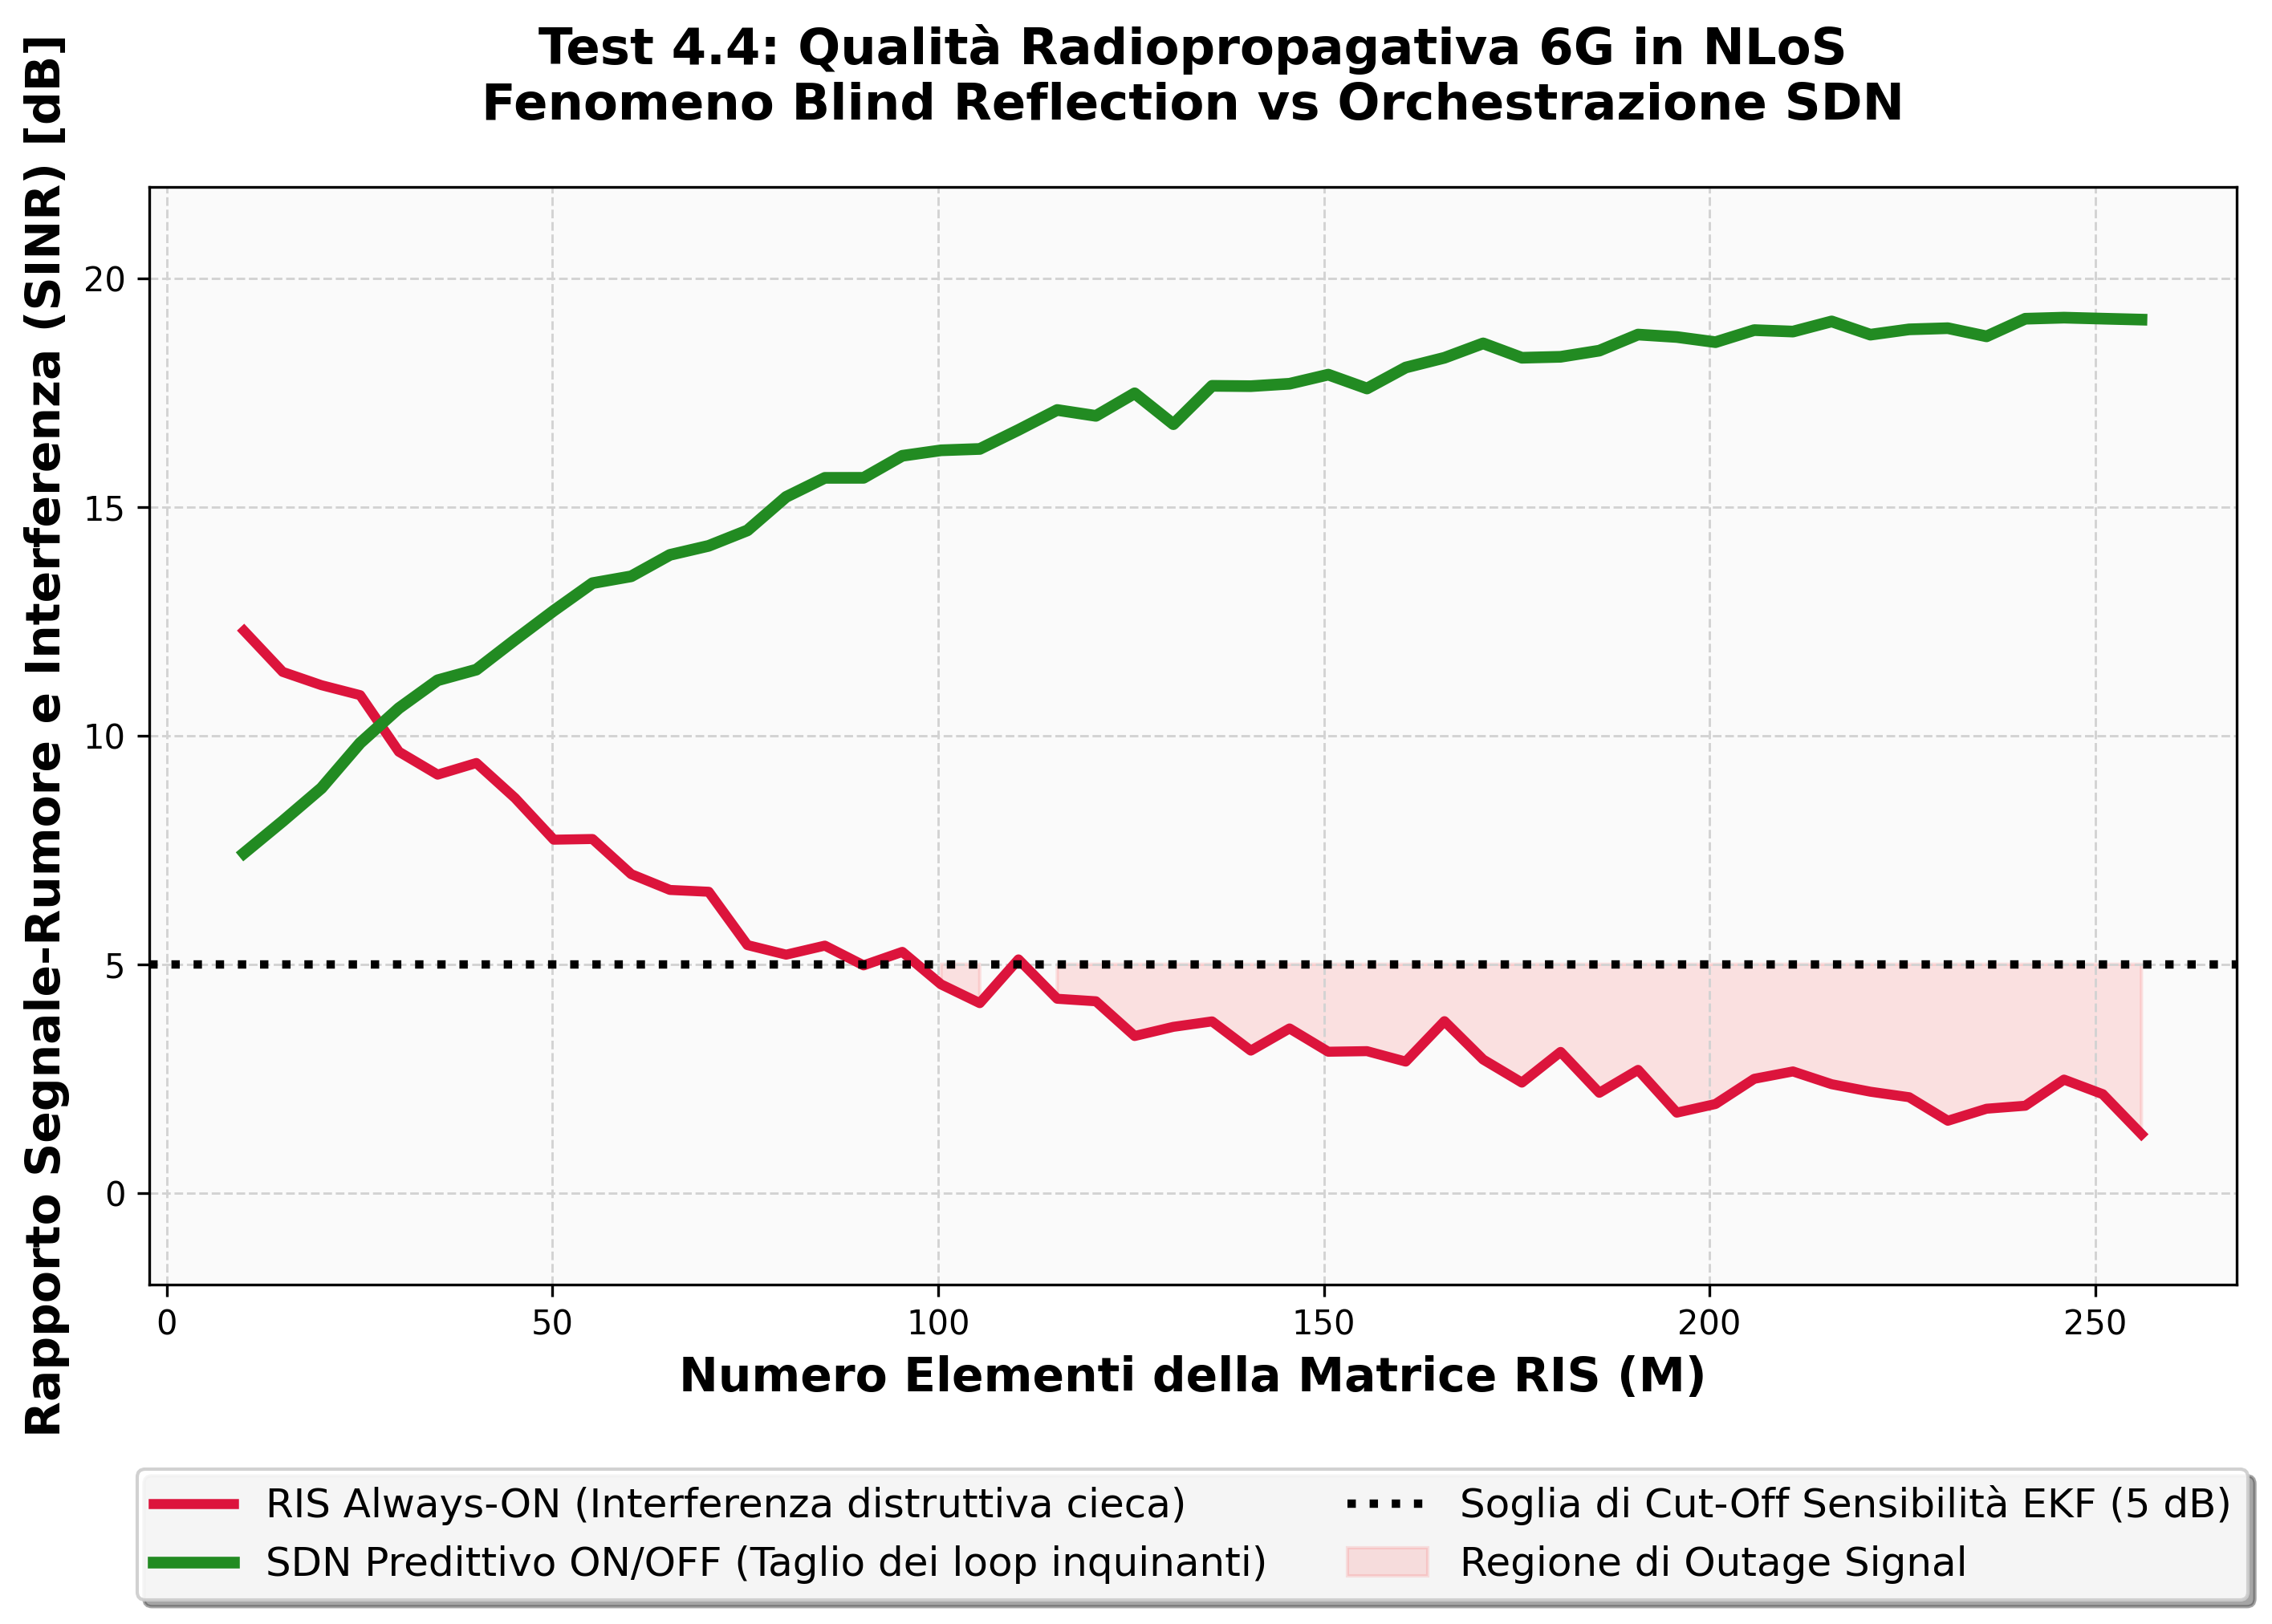
\includegraphics[height=0.7\textheight,keepaspectratio]{Test_4.4_SINR_vs_M_Elements.png}
    \end{center}
\end{frame}

% Slide 15
\begin{frame}{Conclusioni e Sviluppi Futuri}
    \begin{columns}
        \begin{column}{0.6\textwidth}
            \textbf{Obiettivi Raggiunti:}
            \begin{itemize}
                \item Tracking sub-metrico NLoS robusto.
                \item Controller ibrido EKF-LSTM funzionante.
                \item Efficienza termodinamica Green 6G dimostrata.
            \end{itemize}
            \vspace{1em}
            \textbf{Sviluppi Futuri:}
            \begin{itemize}
                \item Integrazione di imperfezioni hardware reali (Phase-Errors).
                \item Gestione simmetrica di interi sciami di droni coordinati.
            \end{itemize}
        \end{column}
        \begin{column}{0.4\textwidth}
            \begin{center}
                % Se \usepackage{fontawesome5} funziona, altrimenti rimuoviamo
                \Large \textbf{Grazie per l'attenzione.}
            \end{center}
        \end{column}
    \end{columns}
\end{frame}

\end{document}
